\documentclass[book.tex]{subfiles}
\begin{document}
\label{chapter_cache_compression}
\section{Asset Caching and Compression}

The floppy disk is not only the slowest component of the PC but also constrained in terms of storage space. Therefore, it is crucial to load and store game assets as efficiently as possible in memory, avoiding long and unnecessary loading times from the disk. To make matters worse, the total amount of assets and maps cannot fit into RAM all at once. This is where a cache manager becomes essential. Its primary purpose is to increase data retrieval performance by reducing the need to load data from the slow floppy disk. 

\subsection{Asset caching}
To manage and track the assets to be loaded into memory, the game engine uses a caching level mechanism. An array, sized according to the total number of graphical assets, is maintained to mark whether an asset needs to be loaded into memory. \\

\lstinputlisting[language=C]{code/cache_structure.c} 
\par
The index of this array corresponds to the graphic asset IDs. Using eight bits, the array can manage the required assets for different cache levels. The \cw{ca\_levelnum} variable points to the current cache level. Upon executing the engine, the cache manager starts with an empty array and \cw{ca\_levelnum} set to 1.\\

\begin{figure}[H]
\centering
\setlength{\tabcolsep}{0pt} % set border margin to 0
\begin{tabular}{m{15em}|S|S|S|S|S|S|S|S|S|} 
  \multicolumn{1}{r|}{\it level bit: \kern 0.15em} & \it 8 & \it 7 & \it 6 & \it 5 & \it 4 & \it 3 & \it 2 & \cellcolor{light_grey} \it 1 \\ \hline
  STARTFONT &  & & & & & & &  \\ \hline
  CTL\_STARTUPPIC &  & & & & & & & \\  \hline
  CTL\_HELPUPPIC &  & & & & & & & \\ \hline
  ... &  & & & & & & & \\ \hline
  KEENSTANDRSPR &  & & & & & & & \\ \hline
  KEENRUNR1SPR &  & & & & & & &  \\ \hline
  ... &  & & & & & & & \\ \hline
  SCOREBOXSPR &  & & & & & & & \\ \hline
  ... &   & & & & & & & \\ \hline
  TILE8 &  & & & & & & & \\  \hline
  TILE8M &  & & & & & & & \\ \hline
  TILE16 \#1 &  & & & & & & & \\ \hline
  TILE16 \#2 &  & & & & & & & \\ \hline
  ... &  & & & & & & & \\ \hline
\end{tabular}\\
\setlength{\tabcolsep}{6pt} % reset border margin
\caption{Initiating \cw{grneeded[]} array, current cache level is 1.}
\end{figure}

When new resources for a level need to be cached in memory, all required assets are marked by setting the current level bit (bit 1). \\

\lstinputlisting[language=C]{code/unrolled_mark_cache.c}

\par
The function \cw{CA\_CacheMarks} then iterates through the cache array, checking if any of the required assets are not yet available in memory. If not, it loads and decompresses the asset from disk into memory.


\begin{figure}[H]
\centering
\setlength{\tabcolsep}{0pt} % set border margin to 0
\begin{tabular}{m{15em}|S|S|S|S|S|S|S|S|S|} 
  \multicolumn{1}{r|}{\it level bit: \kern 0.15em} & \it 8 & \it 7 & \it 6 & \it 5 & \it 4 & \it 3 & \it 2 & \cellcolor{light_grey} \it 1 \\ \hline
  STARTFONT &  & & & & & & & \cellcolor{black} \\ \hline
  CTL\_STARTUPPIC &  & & & & & & &  \\  \hline
  CTL\_HELPUPPIC &  & & & & & & & \\ \hline
  ... &  & & & & & & & \\ \hline
  KEENSTANDRSPR &  & & & & & & & \cellcolor{black} \\ \hline
  KEENRUNR1SPR &  & & & & & & &  \cellcolor{black} \\ \hline
  ... &  & & & & & & & \\ \hline
  SCOREBOXSPR &  & & & & & & & \cellcolor{black} \\ \hline
  ... &   & & & & & & & \\ \hline
  TILE8 &  & & & & & & & \cellcolor{black} \\  \hline
  TILE8M &  & & & & & & & \cellcolor{black} \\ \hline
  TILE16 \#1 &  & & & & & & & \cellcolor{black} \\ \hline
  TILE16 \#2 &  & & & & & & & \\ \hline
  ... &  & & & & & & & \\ \hline
\end{tabular}\\
\setlength{\tabcolsep}{6pt} % reset border margin
\caption{Mark and load assets required for the new map in cache level 1.}
\end{figure}


\par
Now, during gameplay, the user opens the control panel (e.g. to pause the game), which requires to load assets for the control panel into memory. The cache level is increased to level two and for all required control panel assets the second bit is marked.\\

\par
\lstinputlisting[language=C]{code/CA_level_up.c}

\par

The \cw{grneeded[]} cache array then appears as below.\\

\begin{figure}[H]
\centering
\setlength{\tabcolsep}{0pt} % set border margin to 0
\begin{tabular}{m{15em}|S|S|S|S|S|S|S|S|S|} 
  \multicolumn{1}{r|}{\it level bit: \kern 0.15em} & \it 8 & \it 7 & \it 6 & \it 5 & \it 4 & \it 3 & \cellcolor{light_grey} \it 2 & \it 1 \\ \hline
  STARTFONT &  & & & & & & \cellcolor{black} & \cellcolor{black} \\ \hline
  CTL\_STARTUPPIC &  & & & & & & \cellcolor{black} &  \\  \hline
  CTL\_HELPUPPIC &  & & & & & & \cellcolor{black} & \\ \hline
  ... &  & & & & & & & \\ \hline
  KEENSTANDRSPR &  & & & & & & & \cellcolor{black} \\ \hline
  KEENRUNR1SPR &  & & & & & & &  \cellcolor{black} \\ \hline
  ... &  & & & & & & & \\ \hline
  SCOREBOXSPR &  & & & & & & \cellcolor{black} & \cellcolor{black} \\ \hline
  ... &   & & & & & & & \\ \hline
  TILE8 &  & & & & & & \cellcolor{black} & \cellcolor{black} \\  \hline
  TILE8M &  & & & & & & \cellcolor{black} & \cellcolor{black} \\ \hline
  TILE16 \#1 &  & & & & & & & \cellcolor{black} \\ \hline
  TILE16 \#2 &  & & & & & & & \\ \hline
  ... &  & & & & & & & \\ \hline

\end{tabular}\\
\setlength{\tabcolsep}{6pt} % reset border margin
\caption{Mark all assets required for the control panel in cache level 2.}
\end{figure}
\par

\par
The function \cw{CA\_CacheMarks()} is called again to load all cache level 2 assets into memory. It iterates over all assets, loading any missing ones into memory. Any asset that is not required for cache level 2, but is already in memory will be marked for purging, meaning the memory manager can remove it from memory in case of insufficient memory.\\

\lstinputlisting[language=C]{code/unrolled_CA_CacheMarks.c}

\par
In this example, this applies to 
\begin{itemize}
  \item \cw{KEENSTANDRSPR}
  \item \cw{KEENRUNR1SPR}
  \item \cw{TILE16 \#1} 
\end{itemize}

\par
When the user closes the control panel, the engine lowers the cache level back to 1, where all assets required for playing the level are memorized. Simply calling the function \cw{CA\_CacheMarks()} again reloads any assets that were removed from memory.\\

\pagebreak
\lstinputlisting[language=C]{code/CA_level_down.c}
\par
To avoid frequently used assets, such as fonts and Commander Keen sprites, being reloaded every time from the disk, they are loaded permanently into memory by flagging them as non-movable, unpurgeable blocks of memory. \\

\par
\lstinputlisting[language=C]{code/cache_setlock.c}
\par
 
\subsection{Asset compression}
Given that the floppy disk is limited in both speed (100-250 kbps\footnote{Kilobit per second is a unit of data transfer rate equal to: 1,000 bits per second or 125 bytes per second.}) and storage capacity (3\nicefrac{1}{2}-inch disk size is either 720KB or 1.44MB), file compression was essential. Compression ensures that the game occupies less space and loads more quickly. id Software used "Huffman compression" for all asset and map files, with additional "RLE compression" applied to further reduce the size of map files.\\


\par
Huffman compression involves changing how various characters are stored. Normally, all characters in a given segment of data are equal and take an equal amount of space to store. However, by making more common characters take up less space while allowing less commonly used characters to take up more, the overall size of a segment of data can be reduced. \\


\par
To illustrate the various aspects of Huffman compression, the following text, where each character is one byte, will be Huffman compressed: \\


\par
\begin{minipage}{\textwidth}
 \lstinputlisting[language=C]{code/huffman_text}\par
 \end{minipage}

\par
The first step is to make a character frequency table.

\begin{figure}[H]
\centering
{\renewcommand{\arraystretch}{1.2} %<- modify value to suit your needs
\newcolumntype{Y}{>{\centering\arraybackslash}X}
\begin{tabularx}{\textwidth}[c]{|>{\hsize=.22\hsize}Y |>{\hsize=.22\hsize}Y |>{\hsize=.12\hsize}Y |>{\hsize=.22\hsize}Y |>{\hsize=.22\hsize}Y |}
  \cline{0-1}\cline{4-5}
  \textbf{Character} & \textbf{Frequency} & & \textbf{Character} & \textbf{Frequency} \\ 
  \cline{0-1}\cline{4-5}
  e & 6 & & d & 1 \\ 
  n & 4 & & D & 1 \\ 
  space & 4 & & C & 1 \\
  m & 3 & & o & 1 \\
  a & 2 & & i & 1 \\ 
  r & 2 & & s & 1 \\
  K & 2 & & & \\ 
  \cline{0-1}\cline{4-5}
\end{tabularx}
}
\caption{Character frequency table.}
\end{figure}

Next, an optimal binary tree, also known as a dictionary, is created. This is done by starting with the most common character and checking if it occurs more frequently than all the other characters combined. If not, then the second most common character is added, and so on. In our example, four characters make up more than half of the total number of characters: 'e', 'n', space, and 'm'. All of these characters are placed on the left side of the root node, while the remaining characters are placed on the right side.\\

\begin{figure}[H]
\centering
 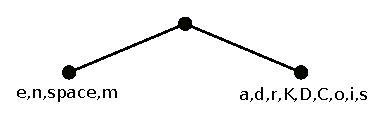
\includegraphics[width=0.5\textwidth]{imgs/drawings/huffman_tree_1.eps}
 \end{figure}

 \par
The process continues by creating a new node with left and right branches and repeating the steps. The two most common characters in the left node, 'e' and 'n', are assigned to the left branch of this new node. A third node is created, and since there are only two options, each is given a branch. This process is applied to the remaining characters of the left node, resulting in the structure shown below. \\

\begin{figure}[H]
\centering
 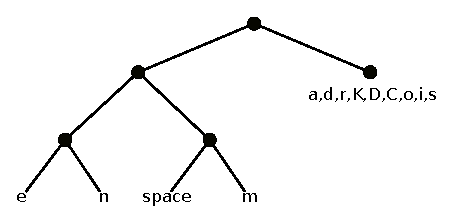
\includegraphics[width=0.6\textwidth]{imgs/drawings/huffman_tree_2.eps}
 \end{figure}

 \par
The same procedure is applied to the right node, where 'a', 'd', 'r', and 'K' constitute more than half of the total number of characters in the right node. After following the same steps, the final binary tree looks as follows:\\
 
\begin{figure}[H]
\centering
 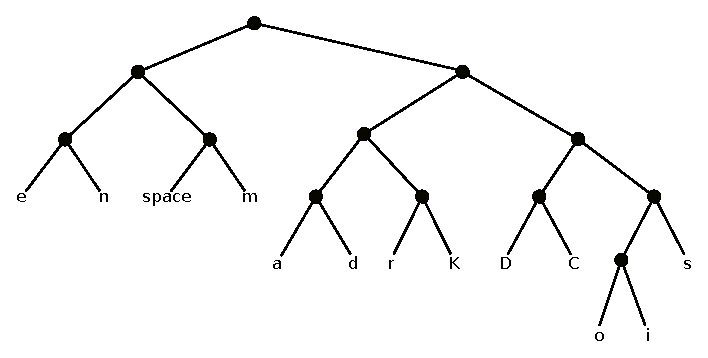
\includegraphics[width=0.9\textwidth]{imgs/drawings/huffman_tree_3.eps}
 \end{figure}

 \par
Now, the entire text can be encoded by moving left (bit 0) or right (bit 1) through the tree, starting from the top node. For example, the character 'e' is \cw{000}, 'm' is \cw{011}, and 'o' is \cw{11100}. The complete compressed message in bit form is now:\\


\begin{figure}[H]
\centering
 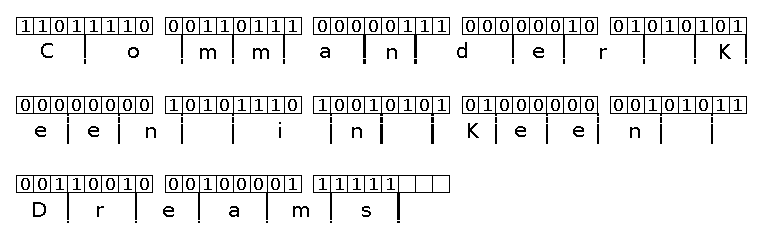
\includegraphics[width=\textwidth]{imgs/drawings/huffman_decode.eps}
 \end{figure}

 \par
This results in a total of 13 bytes used for a 31-byte message, more than a 50\% reduction. In Commander Keen, the dictionary is part of the game engine. Therefore, it is important that the asset files from the shareware version correspond with the dictionary files in the source code\footnote{That's why a specific source code version is mentioned in section "\nameref{section:source_code}" on page \pageref{section:source_code}.}. Reading the Huffman-compressed asset file is straightforward: you read bit by bit from the file and follow the dictionary, starting from the top node, until you reach an end node. The engine then writes the byte to memory and returns to the top node in the dictionary for the next bit in the file.\\

\par
\begin{minipage}{\textwidth}
 \lstinputlisting[language=C]{code/huffman_struct.c}\par
 \end{minipage}\\

\par
The tile map asset files use a second compression technique, on top of Huffman. Upon closer inspection of a level, you'll notice large chunks of the same tile. For example, consider the first level you enter (Horse Radish Hill), which contains extensive areas of blue sky. Here, \textit{Run-length encoding} (RLE) compression comes in useful.\\

\par
The essence of this compression method is to compress data by saving the "run-length" of the encountered values, essentially storing the data as a collection of length/value pairs. To illustrate, the string 'aaaaaaaabbb' could be compressed to '8a3b' (8 bytes of 'a', 3 bytes of 'b'). The trick with RLE is to ensure that the data does not end up becoming larger after processing. For instance, using pure length/value pairs, 'abracadabra' would become '1a1b1r1a1c1a1d1a1b1r1a'.\\

\par
In Commander Keen, this is solved by using a 'tag'. This special tag value instructs the program to take specific action upon encountering it. Every value is passed through unchanged until an RLE tag value is encountered. When this tag is read, instead of directly outputting it like other values, two further values are read. The first indicates the number of times to repeat, and the second represents the value to be repeated. The algorithm used in Commander Keen is based on 16-bits, and therefore is named RLEW, where the 'W' stands for word. The RLEW tag is defined as \cw{ABCDh}.\\

The overall result of applying Huffman and RLEW compression results in almost 65\% file size reduction.\\

\begin{figure}[H]
\centering
{\renewcommand{\arraystretch}{1.2} %<- modify value to suit your needs
\begin{tabularx}{\textwidth}{X X r r }
  \hline
  \textbf{Asset type} & \textbf{filename} & \textbf{Uncompressed size\protect\footnotemark} & \textbf{Compressed size}\\ \hline
  Graphic assets & KDREAMS.EGA & 354,075 bytes & 213,045 bytes \\
  Game levels & KDREAMS.MAP & 417,714 bytes & 65,673 bytes\\ 
  Sound assets & KDREAMS.AUD & 4,572 bytes & 3,498 bytes\\ \hline
  Total &  & 776,361 bytes & 282,216 bytes\\ \hline
\end{tabularx}
}
\end{figure}

\addtocounter{footnote}{-1}
\stepcounter{footnote}
\footnotetext{See Appendix \ref{asset_details} for details per asset file.}


\par
\begin{minipage}{\textwidth}
 \lstinputlisting[language=C]{code/RLEWexpand.c}\par
 \end{minipage}\\
 
 


\end{document}